\documentclass[11pt]{article}
\usepackage{graphicx}
\usepackage{hyperref}
%\usepackage{appendix}
\usepackage{amsmath}
\usepackage{amsthm}
\usepackage{amssymb}
\usepackage{float}
\usepackage{commath}
\usepackage{booktabs}
\renewcommand{\arraystretch}{1.2}
\usepackage{siunitx}
\sisetup{detect-all}
\usepackage{listings}
\usepackage{color} %red, green, blue, yellow, cyan, magenta, black, white
\definecolor{mygreen}{RGB}{28,172,0} % color values Red, Green, Blue
\definecolor{mylilas}{RGB}{170,55,241}
\usepackage[a4paper,margin=20mm]{geometry}
\numberwithin{equation}{section}
\setlength{\parskip}{\baselineskip}
\setlength{\parindent}{0pt}
\hypersetup{
    colorlinks=true,
    linkcolor=black,
    filecolor=black,      
    urlcolor=black,
    citecolor=black
}
\urlstyle{same}
\begin{document}
\title{\textbf{UCL Mechanical Engineering 2020/2021}\\MECH0010 Final Assessment}
\author{NCWT3}
\maketitle
\tableofcontents
\listoffigures
\section{Question 1}
\subsection{a}
\begin{figure}[H]
   \centering
   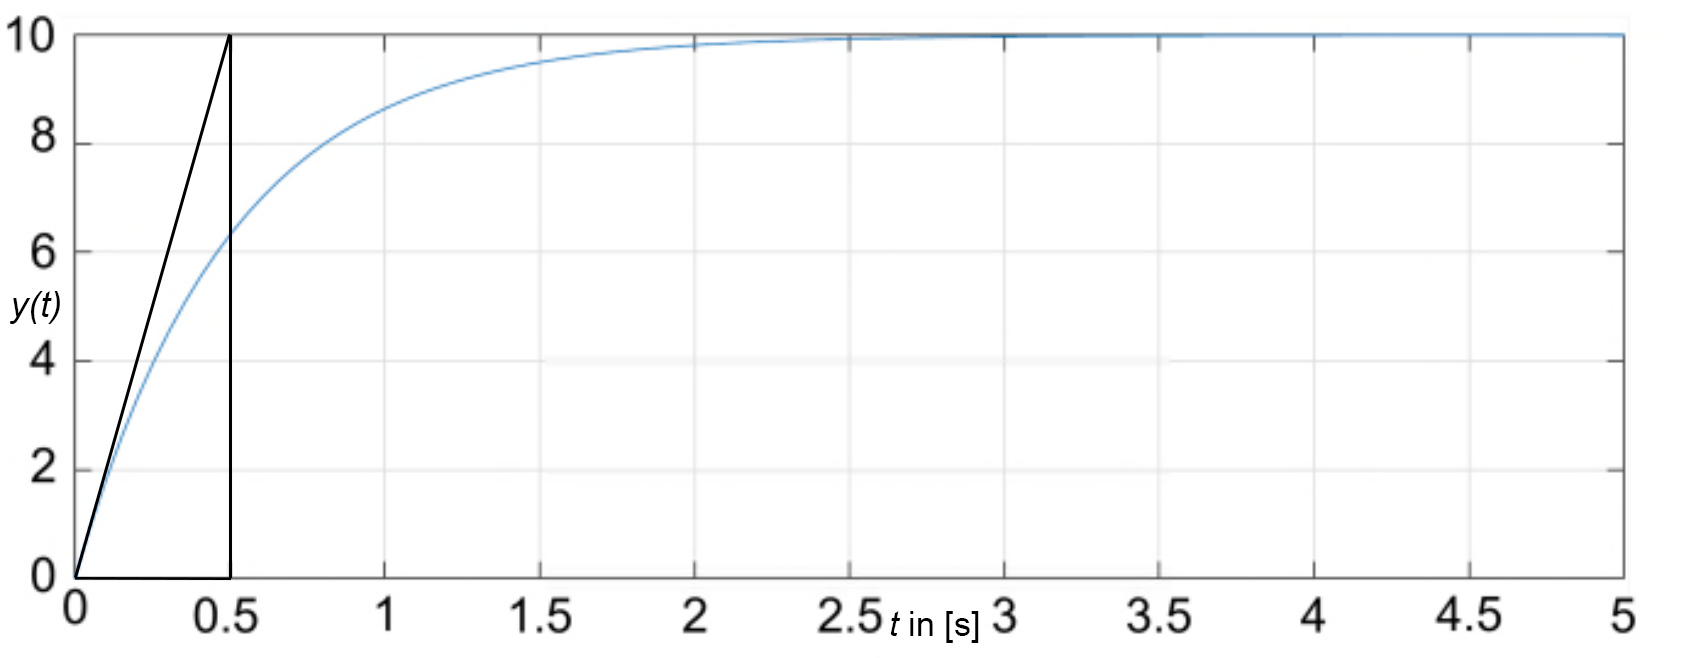
\includegraphics[width = 0.9 \textwidth]{./img/q1i1.png}
   \caption{Diagram to show step response of a first-order system.} 
   \label{fig:q1i1}
\end{figure}
Let us look at \ref{eq:q1i1}
\begin{equation}
    \frac{\dif y(t)}{\dif t} = ay(t) + b u(t)\label{eq:q1i1}
\end{equation}
Transforming to Laplace domain:
\begin{align}
    sY(s) - y(0) &= aY(s) + bU(s)
\end{align}
$y(0) = 0$:
\begin{align}
    Y(s)\left(s-a\right) &= bU(s)\\
    \frac{Y(s)}{U(s)} = \frac{b}{s-a}
\end{align}
For step input $U(s) = \frac{1}{s}$:
\begin{gather}
    Y(s) = \frac{b}{s(s-a)} = \frac{k_1}{s}+ \frac{k_2}{s-a}
\end{gather}
Solving partial fraction:
\begin{gather}
    k_1(s-a) + k_2 s = b\\
    s = 0 \rightarrow -ak_1 = b\\
    k_1 = -\frac{b}{a}\\
    s = a \rightarrow ak_2 = b\\
    k_2 = \frac{b}{a}\\
    Y(s) = \frac{b}{a(s-a)} - \frac{b}{as}\\
    Y(s) = \frac{b}{a}\left(\frac{1}{s-a}-\frac{1}{s}\right)
\end{gather}
Returning to time domain (using tables):
\begin{gather}
    y(t) = \frac{b}{a} \left(e^{at}-1\right) \label{eq:q1i2}\\
    \frac{\dif y(t)}{\dif t} = be^{at}\\
    \left. \frac{\dif y(t)}{\dif t} \right|_{t = 0} = b
\end{gather}
From Figure \ref{fig:q1i1}, we can see that the gradient at 0 is:
\begin{equation}
    b = \frac{10}{0.5} = 20
\end{equation}
Response settles at $y(t) = 10$, therefore:
\begin{align}
    e^{at} &= 0\\
    \therefore 10 &= \frac{20}{a}\left(-1\right)\\
    a &= -2
\end{align}
Hence:
\begin{align}
    y(t) = -10 \left(e^{-2t}-1\right)\\
    \frac{\dif y(t)}{\dif t} = -2y(t) + 10u(t)
\end{align}
\subsection{b}
\subsubsection{i}
\begin{align}
    \frac{\dif \omega(t)}{\dif t} &= -a\omega(t) + kv(t)\\
    s \Omega(s) - \omega(0) &= -a \Omega(s) + kV(s)\\
    s\Omega(s) +a\Omega (s) &= kV(s)\\
    \Omega(s)\left(s+a\right) &= kV(s)\\
    \frac{\Omega (s)}{V(s)} &= \frac{k}{s+a}\\
    \frac{\Omega (s)}{V(s)} &= \frac{\frac{k}{a}}{\frac{s}{a}+1} = \frac{\gamma}{\tau s + 1}
\end{align}
Where $\gamma$ is the gain and $\tau$ is the time constant.
\section{Question 2} 
In order to take a measurement of the air flow in the pipe, we will be utilising a temperature based measurement from a hot wire anemometer. The working principle of a hot wire anemometer is to measure the changes in current of the wire, as air flow past the wire changes its temperature. The wire is heated to a temperature above the ambient through a constant voltage. Current flow increases the temperature of the wire, increasing the electrical resistance. As air flows past the wire, temperature decreases, decreasing electrical resistance. However, this will increase the current for constant voltage and the resistance of the wire will reach equilibrium once again. 
\end{document}